\chapter{Principes de l’édition}\label{ch:edition}

\section{Niveaux de contrôle des lectures}

Chaque notice indique le statut de son texte selon une échelle de contrôle explicite. Les trois premiers niveaux ne sont atteints par aucune notice ; ils sont nommés pour que le lecteur sache ce qui n’a pas été fait.

\begin{description}[style=nextline,leftmargin=1.5em,font=\normalfont\scshape]
\item[Lecture contrôlée sur le monument] Texte vérifié par autopsie. Aucune notice.
\item[Lecture contrôlée sur photographie] Texte comparé à une photographie authentifiée et identifiable, en entier. Aucune notice ; deux notices ont fait l’objet d’un contrôle partiel sur reproduction (\nnums{38} et 68).
\item[Lecture d’après l’édition imprimée] Texte comparé à l’édition effectivement examinée. Aucune notice : les volumes des ICUR, du CIL et de l’ILCV n’ont pas pu être consultés.
\item[Lecture stabilisée entre deux bases] Texte de l’EDCS concordant avec celui de l’EDB aux conventions de notation près, éventuellement après relecture de la fiche détaillée. \st{edbConcTotC} textes funéraires.
\item[Lecture secondaire avec écarts] Texte de l’EDCS présentant des écarts ou une divergence forte avec l’EDB. Les écarts sont décrits dans la notice.
\item[Lecture secondaire sans second témoin] Texte de l’EDCS non apparié à l’EDB.
\end{description}

Une lecture stabilisée n’est pas une lecture validée : les deux bases dépendent de l’ICVR. Elle signifie seulement que deux équipes, travaillant indépendamment sur la même édition, transmettent le même texte.

\section{Conventions de transcription}

Le texte est reproduit ligne par ligne d’après l’état 2022 de l’EDCS, avec les signes diacritiques de la base convertis selon le système de Krummrey et Panciera\footnote{H. Krummrey, S. Panciera, « Criteri di edizione e segni diacritici », \emph{Tituli}, 2, 1980, p. 205–215 (référence et valeur des signes vérifiées sur l’annexe des EpiDoc Guidelines consacrée à ce système).}. La base emploie une notation propre pour les lettres gravées par erreur et corrigées par l’éditeur (\texttt{<a=B>}) ; elle est rendue par les demi-crochets du système Krummrey–Panciera, la lettre effectivement gravée étant donnée en apparat.

\begin{table}[tbp]\centering\small
\caption{Signes diacritiques : notation de l’EDCS et rendu dans ce volume.}\label{tab:signes}
\begin{tabular}{@{}l l l@{}}\toprule EDCS & Ce volume & Valeur\\\midrule
abc(def) & abc(def) & abréviation développée par l’éditeur\\
{[}abc{]} & {[}abc{]} & lettres perdues restituées par l’éditeur\\
{[}3{]} & {[}- - -{]} & lacune d’étendue indéterminée\\
{[}6{]} & - - - - - - & ligne(s) perdue(s), nombre indéterminé\\
\texttt{<v=B>} & ⸢v⸣ & lettre gravée par erreur (B), corrigée par l’éditeur (v)\\
\{abc\} & \{abc\} & lettres superflues gravées\\
(!) & (!) & forme anomale signalée par l’éditeur (\emph{sic})\\
(?) & (?) & lecture ou développement incertain\\
/ & numéro de ligne & changement de ligne\\
// & ‖ & changement de face ou de champ\\\bottomrule
\end{tabular}
\end{table}

Les textes de l’EDB sont cités avec leurs propres conventions : ⟨~⟩ pour les lettres ajoutées par l’éditeur, ⌜~⌝ pour les lettres corrigées, lettres soulignées pour les lettres vues par un éditeur antérieur et aujourd’hui perdues, lettres pointées pour les lectures incertaines, \emph{((monogramma Christi))} et formules analogues pour les signes figurés. Deux signes de balisage interne de la base (\% et £), dépourvus de valeur épigraphique, sont omis. Les mentions « texte tronqué dans la liste de résultats » signalent les textes que la liste publique de l’EDB coupe ; la partie manquante n’est pas reconstituée.

\begin{figure}[tbp]\centering
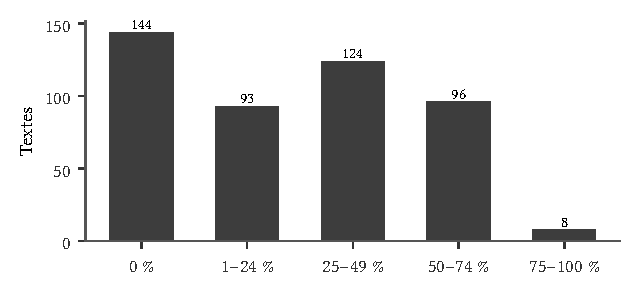
\includegraphics[width=0.7\linewidth]{figures/fig_restitution.pdf}
\caption{Part des lettres restituées déclarée par la base pour les textes de l’ensemble C (n = \st{nC}). Ces pourcentages ne mesurent pas la surface perdue des monuments.}\label{fig:restitution}
\end{figure}

La part des restitutions varie fortement d’un texte à l’autre (figure~\ref{fig:restitution}) : \st{nZeroRest} textes funéraires n’en comportent aucune, \st{nPlusMoitie} sont restitués pour plus de moitié. Pour ces derniers, toute observation linguistique ou religieuse est conditionnelle.

\section{Traductions}

Les traductions sont des traductions de travail. Elles suivent le texte au plus près ; les lacunes sont rendues par […], les sens incertains par un point d’interrogation entre parenthèses. Elles traduisent souvent des parties restituées par l’éditeur : le lecteur doit se reporter au texte pour distinguer ce qui est lu. Elles n’ont pas encore été relues par un spécialiste ; cette relecture, par un latiniste et un helléniste, est une condition de la publication.

\section{Structure des notices}

Chaque notice du catalogue suit le même ordre. Les rubriques sans objet sont omises.

\begin{description}[style=nextline,leftmargin=1.5em,font=\normalfont\scshape]
\item[En-tête] Numéro stable, année de classement, première référence ICUR, identifiants EDCS, EDB et, le cas échéant, EDH.
\item[Datation] Année et fondement : nom consulaire lu, lu en partie, réduit à des initiales ou restitué ; formule transmise par l’EDB ; restitution conjecturale ; attribution de la base. La mention « datation contestée » renvoie à la rubrique Chronologie.
\item[Genre] Genre épigraphique, appartenance aux ensembles B et C, nombre de lettres et part restituée.
\item[Références] Concordances transmises par l’EDCS, sous une forme normalisée. Elles n’ont pas été vérifiées sur les volumes.
\item[Provenance] Rattachement topographique et lieu de conservation selon l’EDB, cités dans la forme de la base.
\item[Support] Type de support, matériau, dimensions, technique d’exécution, signes figurés, caractère métrique et reproductions disponibles selon la fiche EpiDoc de l’EDB, avec le nom de son rédacteur.
\item[Texte] Texte de l’EDCS (état 2022), ligne par ligne.
\item[Témoins] Différences avec l’export de 2020 ; texte de l’EDB lorsqu’il diffère ; relecture des fiches détaillées ; décisions sur les doublons et les fragments.
\item[Apparat] Lettres gravées corrigées par l’éditeur, lettres superflues, formes signalées.
\item[Traduction] Traduction de travail.
\item[Langue, Chronologie, Commentaire] Observations linguistiques ; noms consulaires et leur état de lecture, faux consuls, dates du jour, âges, divergences ; vocabulaire religieux et renvoi au dossier commenté.
\item[Bibliographie] Références d’édition et bibliographie complémentaire donnée par l’EDB.
\item[Statut] Niveau de contrôle de la lecture.
\end{description}

Une épitaphe brève n’est pas artificiellement développée. Les dossiers commentés (chapitre~\ref{ch:dossiers}) complètent les notices dont les difficultés exigent une discussion.
